
% Eigener Beitrag: Beschreibung, Begründung, Aufzeigung, Methode, Fazit

\chapter{Anforderungen und Analyse}
\label{sec:analyse}

Es gibt folgende Anforderungen an die Testsuite:
\begin{figure}[H]
	\centering
	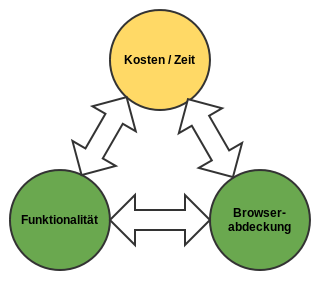
\includegraphics[width=0.6\textwidth]{images/triangle.png}
	\caption{Anforderungsdreieck}
	\label{fig:analyse:Anforderungsdreieck}
\end{figure}

Je mehr Funktionalität abgedeckt wird, desto länger dauern die Test. Und für jeden Browser müssen nochmals alle Tests durchgeführt werden. Deshalb stehen "`Kosten / Zeit"' im Widerspruch mit der Funktionalität und der Browserabdeckung.

Diese Anforderungen sind in den nächsten Abschnitten beschrieben.

\section{Funktionalität}
\label{sec:analyse:Funktionalität}
Die gesamte Funktionalität der Webseite, inklusive der Priorisierung, ist im \cref{app:Funktionalitäten} \nameref{app:Funktionalitäten} aufgelistet. Die Liste wurde im Wiki von der Hotelplan Management AG erstellt. Diese soll auch nach der Arbeit weiter gepflegt werden und wurde deshalb so aufgebaut, dass sie sehr Übersichtlich ist und einfach bearbeitet und erweitert werden kann.

Vor dieser Arbeit gab es keine Dokumente, welche die Funktionalität der Webseite beschrieb. Deshalb musste die gesamte Funktionalität durch analyse der bestehenden Seite rekonstruiert werden (reverse engineering).

\section{Browserabdeckung}
Im \cref{sec:Recherche:TestingFrameworks:Prototyp} \nameref{sec:Recherche:TestingFrameworks:Prototyp} sind die meist verwendeten Browser aufgelistet. Der Vorteil an den Service-Anbietern ist, dass es sehr leicht ist eine Testsuite auf einem weiteren Webbrowser auszuführen. Es ist zu eruieren wie lange die Tests brauchen um durchzulaufen. Dann kann entschieden werden, im Betracht der Kosten, auf wie vielen Browsern die Testsuite durchgeführt wird. Diese Entscheidung wird mit dem Business der Travelwindow AG getroffen, da sie den Kostenrahmen der Tests bestimmen.

\section{Kosten \& Zeit}
Kosten \& Zeit sind wichtig, da die Tests oft gestartet werden müssen und deshalb nicht zu lange dauern sollten. Die Service-Anbietern rechnen pro Minute ab, welche die Tests auf ihren Systemen laufen. 

Für jeden Test wird eine neue \Gls{glos:virtualMachine} gestartet, was Zeit beansprucht. Deshalb wird versucht, die Anzahl der Testfälle zu minimieren, um trotzdem die gesamte Funktionalität abdecken zu können.

Je nachdem wie lange die Tests benötigen kann über die Anzahl der Browser, auf denen die Tests laufen gelassen werden sollen, die Kosten gesteuert werden.